\chapter{Test Problem}
\label{chap:testprob}

A simple test problem is described in this section.
Diagrams of the forward, adjoint, and contributon flux as well as the forward and adjoint current were produced to give insight into the physics of the test problem.
$\delta R\left(\vec{r}\right)$ was then calculated for several perturbations.

% The results were checked against MCNP results to verify that the method used to calculate $\delta R$ is correct.

%%%%%%%%%%%%%%%%%%%%%%%%%%%%%%%%%%%%%%%%%%%%%%%%%%%%%%%%%%%%%%%%%%%%%%%%%%%%%%%%
\section{Test Problem Overview}
\label{sec:bg:tp:overview}
%%%%%%%%%%%%%%%%%%%%%%%%%%%%%%%%%%%%%%%%%%%%%%%%%%%%%%%%%%%%%%%%%%%%%%%%%%%%%%%%

The test problem consists of an accelerator-based DD fusion neutron source (around 2.45 MeV), a tally region in which it is desired to maximize the ${}^{235}\text{U}$ fission rate, a moderating region, and an iron wall to separate the moderator from the tally region.
The goal of the test problem is to find the configuration of materials in the moderating region the produces the highest tally result.

The ``baseline'' moderator configuration is that it is entirely comprised of light water.
All other configurations will be compared to the baseline.
A diagram of the baseline test problem geometry is shown in Figure \ref{fig:tp:material_map}.

\begin{figure}[h!]
  \centering
  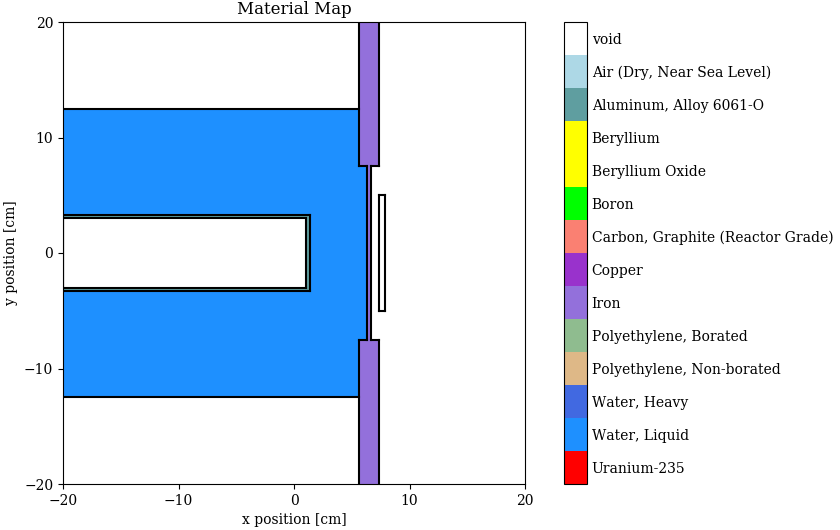
\includegraphics[width=\linewidth]{content/testprob/material_map.png}
  \caption{Material map for test problem.}
  \label{fig:tp:material_map}
\end{figure}

The geometry is entirely comprised of rectangular parallelepipeds (RPPs in MCNP) to avoid there being mesh elements with mixed materials.
In ADVANTG, the 3D spatial mesh has 43 elements in the x-direction and 44 elements in both the y- and z-directions for a total of 83,248 voxels.

The ``27n19g'' multigroup cross section library, which contains 27 neutron energy groups and 19 gamma energy groups, was used.
Since the first two neutron energy groups in this library are above 2.45 MeV, they are unused, leaving 25 neutron energy groups.
Since the tally is a neutron tally and the library does not account for photonuclear reactions, all of the gamma groups are also unused, leaving 25 total energy groups.
Upscattering was explicitly turned off for this analysis to decrease computation time.

The quadrupole range quadrature set with an order of 10 was used.
There were 4 azimuthal and 4 polar directions per octant, for a total of 16 directions per octant, or 128 directions overall.

The forward angular flux thus has $83,248 \times 25 \times 128 = 266,393,600$ values.
Even in this small test problem, the angular forward and adjoint fluxes take up about 4 GB of storage space.

The locations of the energy-integrated source and response are shown in Figures \ref{fig:tp:source_total} and \ref{fig:tp:response_total}.
The source and response energy spectra are shown in \ref{fig:tp:spectra_lin}.
The source energy spectrum is spans the range between 1.97 and 3.23 MeV.
The response energy spectrum is equivalent to the ${}^{235}\text{U}$ fission cross section, which is highest at thermal energies.

\begin{figure}
  \centering
  \begin{minipage}{0.49\linewidth}
    \centering
    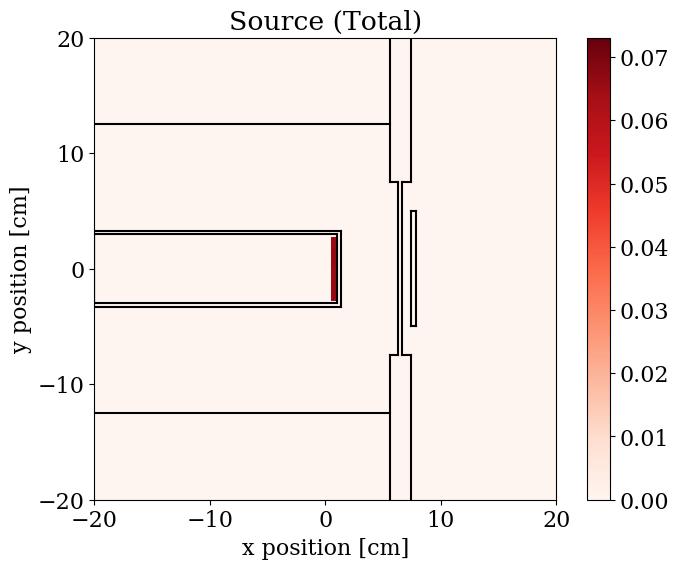
\includegraphics[width=\linewidth]{content/testprob/source_total.png}
    \caption{Location of energy-integrated source in test problem.}
    \label{fig:tp:source_total}
  \end{minipage}
  \hfill
  \begin{minipage}{0.49\linewidth}
    \centering
    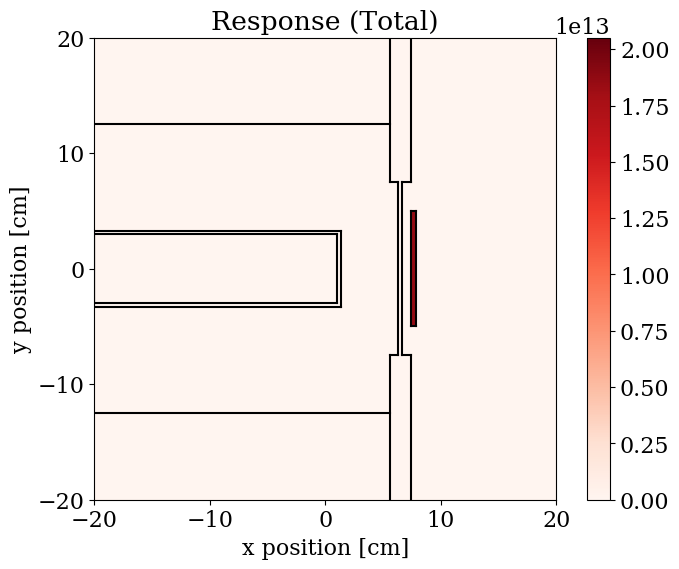
\includegraphics[width=\linewidth]{content/testprob/response_total.png}
    \caption{Location of energy-integrated response in test problem.}
    \label{fig:tp:response_total}
  \end{minipage}
\end{figure}
\begin{figure}
  \centering
  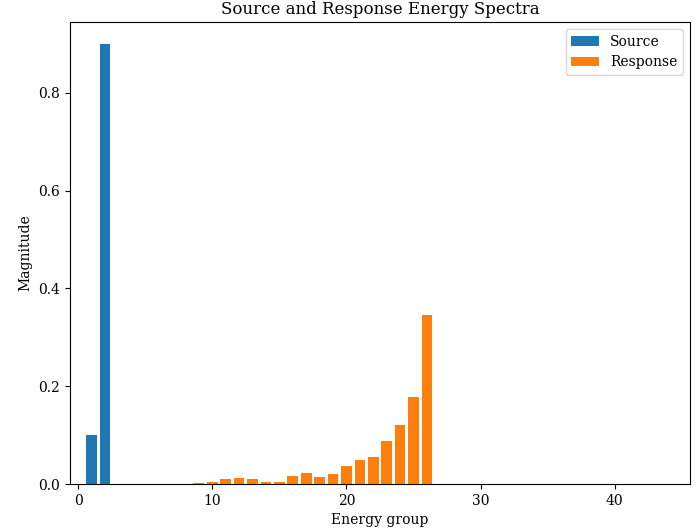
\includegraphics[width=0.5\linewidth]{content/testprob/spectra_lin.png}
  \caption{Source and response energy spectra in test problem.}
  \label{fig:tp:spectra_lin}
\end{figure}

%%%%%%%%%%%%%%%%%%%%%%%%%%%%%%%%%%%%%%%%%%%%%%%%%%%%%%%%%%%%%%%%%%%%%%%%%%%%%%%%
\section{Flux and Current in Test Problem}
\label{sec:bg:tp:flux}
%%%%%%%%%%%%%%%%%%%%%%%%%%%%%%%%%%%%%%%%%%%%%%%%%%%%%%%%%%%%%%%%%%%%%%%%%%%%%%%%

% Note: first energy group should probably be group 1, not group 2.

The scalar forward flux and forward current for energy group 2 (1.8268 to 3.0119 MeV) are shown in Figures \ref{fig:tp:scalar_flux_fwd_g02} and \ref{fig:tp:current_fwd_g02}.
The plots clearly show that fast neutron flux is highest close to the source, with fast neutrons radiating outward from that location.
Ray effects, which are caused by the angular discretization, are clearly visible in the plot of the scalar forward flux.

\begin{figure}
  \begin{minipage}{0.49\linewidth}
    \centering
    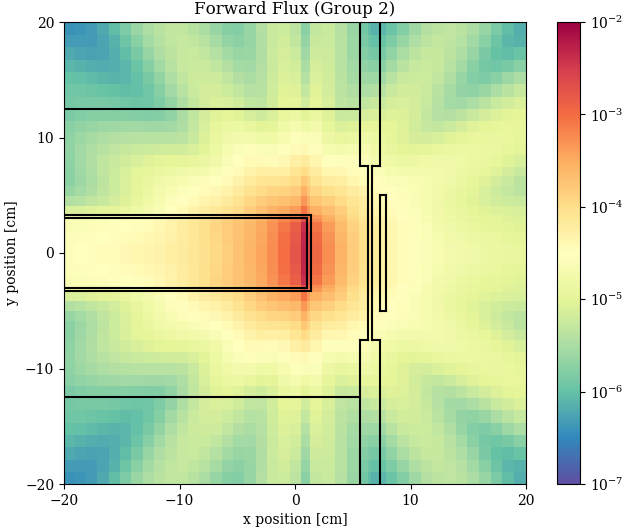
\includegraphics[width=\linewidth]{content/testprob/scalar_flux_fwd_g02.png}
    \caption{Scalar forward flux in energy group 2 in test problem.}
    \label{fig:tp:scalar_flux_fwd_g02}
  \end{minipage}
  \hfill
  \begin{minipage}{0.49\linewidth}
    \centering
    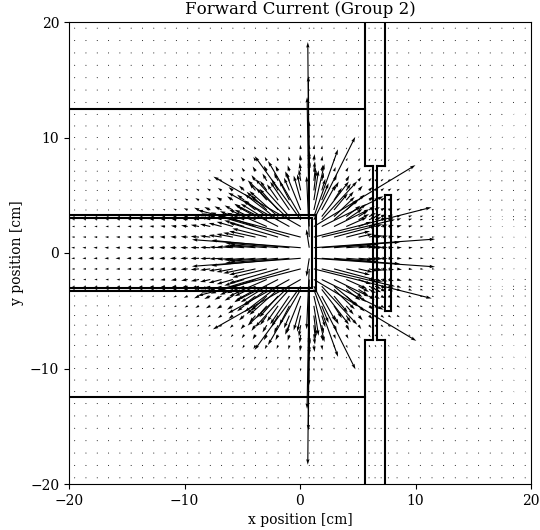
\includegraphics[width=\linewidth]{content/testprob/current_fwd_g02.png}
    \caption{Forward current in energy group 2 in test problem.}
    \label{fig:tp:current_fwd_g02}
  \end{minipage}
\end{figure}

The scalar forward flux and forward current for for energy group 26 ($10^{-11}$ to $10^{-8}$ MeV) are shown in Figures \ref{fig:tp:scalar_flux_fwd_g26} and \ref{fig:tp:current_fwd_g26}.
The plots show that the thermal neutron population is significantly mores spread out, existing as a cloud that encompasses most of the moderating region.
The thermal neutron flux is mostly isotropic within the moderating region.

\begin{figure}
  \begin{minipage}{0.49\linewidth}
    \centering
    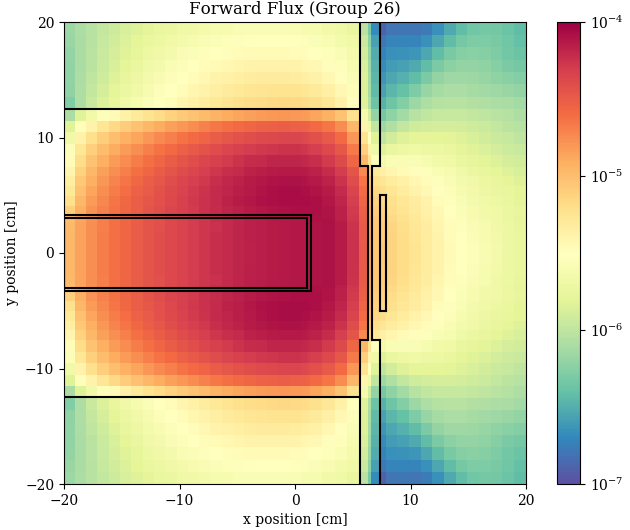
\includegraphics[width=\linewidth]{content/testprob/scalar_flux_fwd_g26.png}
    \caption{Scalar forward flux in energy group 26 in test problem.}
    \label{fig:tp:scalar_flux_fwd_g26}
  \end{minipage}
  \hfill
  \begin{minipage}{0.49\linewidth}
    \centering
    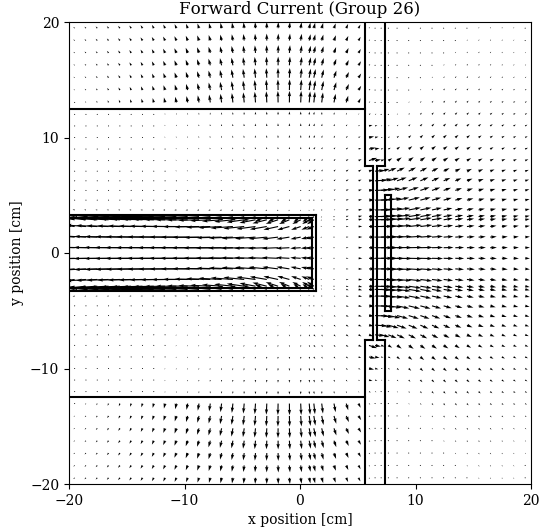
\includegraphics[width=\linewidth]{content/testprob/current_fwd_g26.png}
    \caption{Forward current in energy group 26 in test problem.}
    \label{fig:tp:current_fwd_g26}
  \end{minipage}
\end{figure}

% The scalar adjoint flux for energy groups 2 and 26 are shown in Figures \ref{fig:tp:scalar_flux_adj_g02} and \ref{fig:tp:scalar_flux_adj_g26}.
% The group 26 adjoint flux shows that thermal neutrons close to the detector have a high likelihood of contributing to the detector.
% The group 2 adjoint flux shows that fast neutrons have the highest likelihood of contributing to the detector while they are still in the moderating region.
% This is because they are more likely to scatter down to thermal energies and then contribute to the detector than they are to immediately contribute to the detector as fast neutrons.

The scalar adjoint flux and adjoint current for energy group 2 are shown in Figures \ref{fig:tp:scalar_flux_adj_g02} and \ref{fig:tp:current_adj_g02}.
The plots show that the region with the highest adjoint flux for fast neutrons is the region in between the source and detector, rather than at the detector itself.
This is an interesting result becuause it indicates that it is more likely that fast neutrons in the moderating region will thermalize and then contribute to the detector than it is that fast neutron already in the detector will contribute to it.
This effect is entirely due to the fact that ${}^{235}\text{U}$ has a fission cross section many orders of magnitude higher at thermal energies than it does at fast energies.

\begin{figure}
  \begin{minipage}{0.49\linewidth}
    \centering
    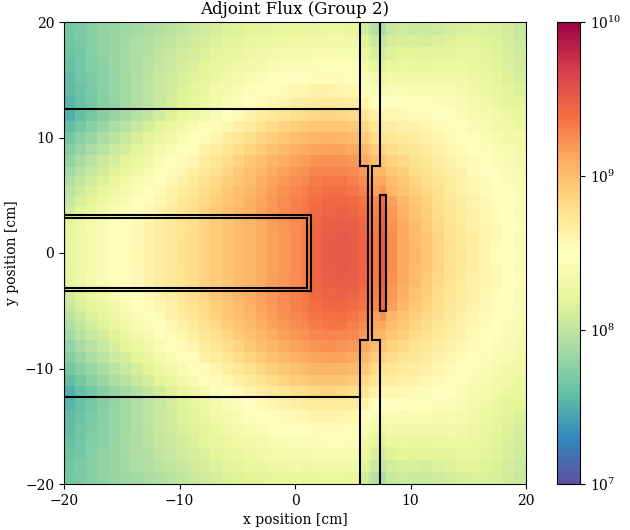
\includegraphics[width=\linewidth]{content/testprob/scalar_flux_adj_g02.png}
    \caption{Scalar adjoint flux in energy group 2 in test problem.}
    \label{fig:tp:scalar_flux_adj_g02}
  \end{minipage}
  \hfill
  \begin{minipage}{0.49\linewidth}
    \centering
    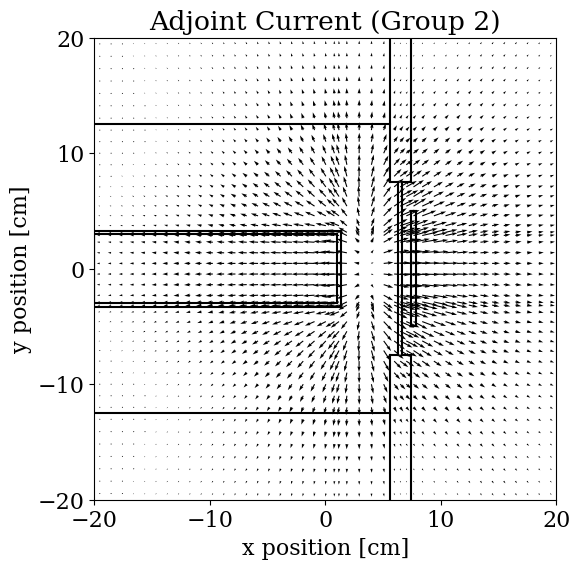
\includegraphics[width=\linewidth]{content/testprob/current_adj_g02.png}
    \caption{Adjoint current in energy group 2 in test problem.}
    \label{fig:tp:current_adj_g02}
  \end{minipage}
\end{figure}

% The adjoint current for energy groups 2 and 26 are shown in Figures \ref{fig:tp:current_adj_g02} and \ref{fig:tp:current_adj_g26}.
% The adjoint current shows the net directionality of the adjoint flux.
% Adjoint fast neutrons do not show strong directionality.
% Adjoint thermal neutrons radiate outward from the detector.

The scalar adjoint flux and adjoint current for energy group 26 are shown in Figures \ref{fig:tp:scalar_flux_adj_g26} and \ref{fig:tp:current_adj_g26}.
The plots clearly show that the adjoint thermal flux radiates outward from the detector.
This means that the closer a thermal neutron is to the detector, the more likely it is to contribute.

\begin{figure}
  \begin{minipage}{0.49\linewidth}
    \centering
    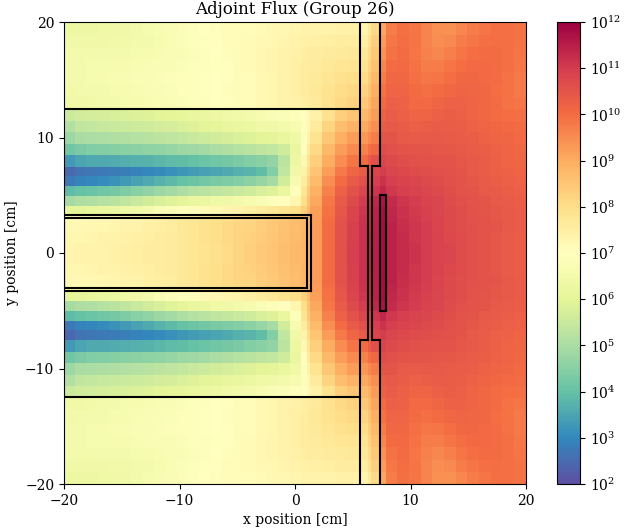
\includegraphics[width=\linewidth]{content/testprob/scalar_flux_adj_g26.png}
    \caption{Scalar adjoint flux in energy group 26 in test problem.}
    \label{fig:tp:scalar_flux_adj_g26}
  \end{minipage}
  \hfill
  \begin{minipage}{0.49\linewidth}
    \centering
    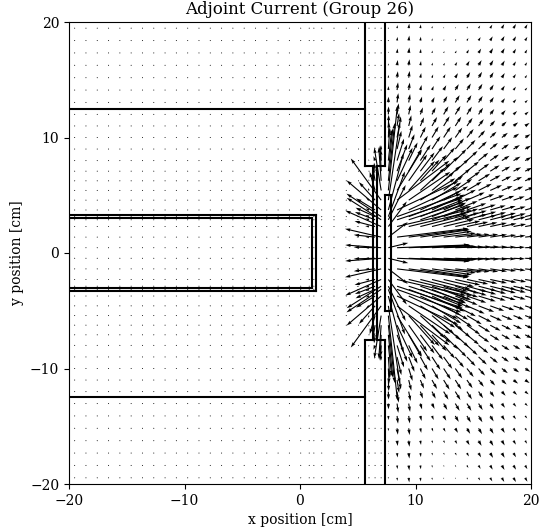
\includegraphics[width=\linewidth]{content/testprob/current_adj_g26.png}
    \caption{Adjoint current in energy group 26 in test problem.}
    \label{fig:tp:current_adj_g26}
  \end{minipage}
\end{figure}

The scalar contributon flux for energy groups 2 and 26 are shown in Figures \ref{fig:tp:scalar_flux_con_g02} and \ref{fig:tp:scalar_flux_con_g26}, and the scalar energy-integrated contributon flux is shown in Figure \ref{fig:tp:scalar_flux_con_total}.
Equation \ref{eq:bg:rt:scalar-contributon}, repeated here:
\begin{equation*}
  \Phi\left(\vec{r},E\right) \equiv
  \int_{4\pi}\psi\left(\vec{r},\hat{\Omega},E\right)\psi^+\left(\vec{r},-\hat{\Omega},E\right)d\hat{\Omega}.
\end{equation*}
defines the scalar contributon flux.
The contributon flux is at its highest in the region between the source and detector, which makes sense intuitively.
The physical interpretation of this result is that the region between the source and detector is the ``most important'' region of the problem.

Since the region on the right side of the problem is void, all forward and adjoint particles in that region are traveling to the right.
This is evident in Figures \ref{fig:tp:current_fwd_g02}, \ref{fig:tp:current_fwd_g26}, \ref{fig:tp:current_adj_g02}, and \ref{fig:tp:current_adj_g26}: all current vectors in the void region on the right side of the problem are aiming to the right in some manner; none are aiming left.
Thus, after noting that the directionality of the adjoint flux is reversed in the equation for the contributon flux, the contributon flux in that region is zero.

\begin{figure}
  \begin{minipage}{0.49\linewidth}
    \centering
    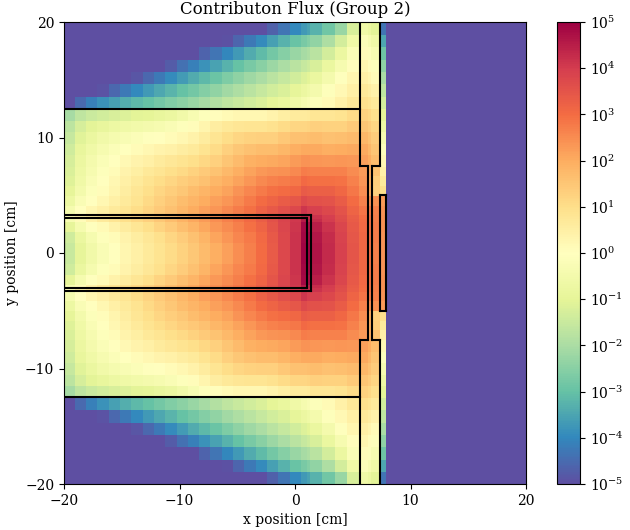
\includegraphics[width=\linewidth]{content/testprob/scalar_flux_con_g02.png}
    \caption{Contributon flux in energy group 2 in test problem.}
    \label{fig:tp:scalar_flux_con_g02}
  \end{minipage}
  \hfill
  \begin{minipage}{0.49\linewidth}
    \centering
    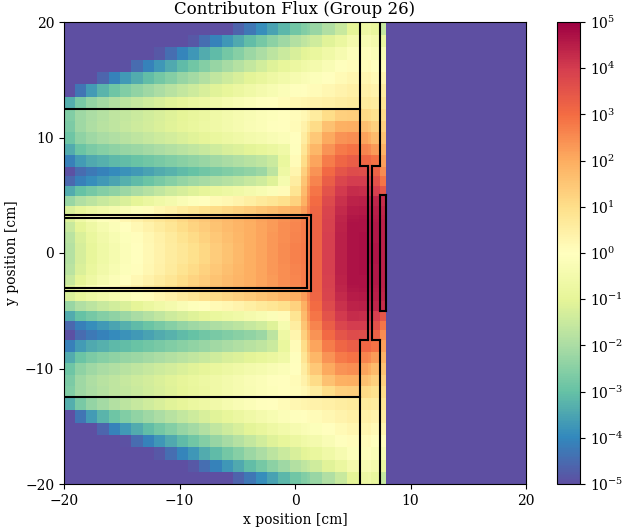
\includegraphics[width=\linewidth]{content/testprob/scalar_flux_con_g26.png}
    \caption{Contributon flux in energy group 26 in test problem.}
    \label{fig:tp:scalar_flux_con_g26}
  \end{minipage}
\end{figure}
\begin{figure}
  \centering
  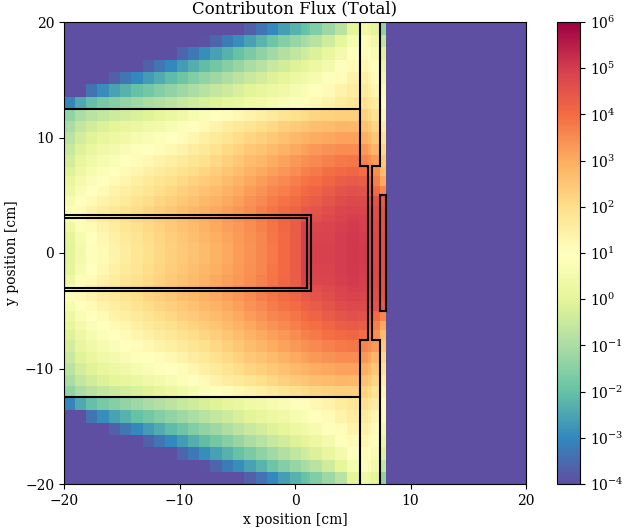
\includegraphics[width=0.5\linewidth]{content/testprob/scalar_flux_con_total.png}
  \caption{Energy-integrated contributon flux in test problem.}
  \label{fig:tp:scalar_flux_con_total}
\end{figure}

%%%%%%%%%%%%%%%%%%%%%%%%%%%%%%%%%%%%%%%%%%%%%%%%%%%%%%%%%%%%%%%%%%%%%%%%%%%%%%%%
\section{Calculation of $\delta R$ in Test Problem}
\label{sec:bg:tp:dr}
%%%%%%%%%%%%%%%%%%%%%%%%%%%%%%%%%%%%%%%%%%%%%%%%%%%%%%%%%%%%%%%%%%%%%%%%%%%%%%%%

Equation \ref{eq:dr:dr_pos_final}, repeated here:
\begin{multline*}
  \delta R\left(\vec{r}\right) =
  \int_0^\infty\phi^+\left(\vec{r},E\right)\left(\int_0^\infty\delta\sigma_s\left(\vec{r},E^\prime\rightarrow E\right)\phi\left(\vec{r},E^\prime\right)dE^\prime\right)dE - \\
  \int_0^\infty\delta\sigma_t\left(\vec{r},E\right)\Phi\left(\vec{r},E\right)dE,
\end{multline*}
was used to calculate $\delta R$ in the test problem.
The value of $\delta R$ at point $\vec{r}_0$; i.e. $\delta R\left(\vec{r}_0\right)$, refers to the perturbation in the detector response given a perturbation in the cross sections ($\delta \sigma_t$ and $\delta \sigma_s$) that only occurs at point $\vec{r}_0$.
The vector quantity $\delta R\left(\vec{r}\right)$ is constructed by calculating $\delta R\left(\vec{r}_0\right)$ for the entire problem domain.

In the test problem, the perturbation is defined as the difference in cross sections between some new material and the existing material.
$\delta R\left(\vec{r}\right)$ was calculated for several different materials, which are listed in Table \ref{tab:testprob:material_list}.
The materials are separated into several categories:
\begin{enumerate}
  \item Low-density: these materials have low or zero density, and are expected to perform poorly as replacement moderators.
  \item Moderating:  these materials are all used as moderators in real-world nuclear systems, so they are expected to perform the best of all materials.
  \item Structural:  these materials are commonly used for structural purposes and are not good moderators, so they are expected to perform poorly.
  \item Absorbing:   these materials are known absorbers of thermal neutrons, so they are expected to perform the the worst.
  \item Fissile:     these materials are neutron multipliers, which means they should perform well in theory, but since the cross section libraries available in ADVANTG do not take fission into account, the results are expected to be poor.
\end{enumerate}

\begin{table}[h]
  \centering
  \caption{List of materials considered in the test problem.}
  \label{tab:testprob:material_list}
  \begin{tabular}{| c | c | c |}
    \hline
    \textbf{Material}  & \textbf{Group}       \\ \hline
    Void               & Low-density          \\ \hline
    Air                & Low-density          \\ \hline
    Beryllium oxide    & Moderating           \\ \hline
    Graphite           & Moderating           \\ \hline
    Light water        & Moderating           \\ \hline
    Heavy water        & Moderating           \\ \hline
    HDPE               & Moderating           \\ \hline
    Borated HDPE       & Moderating/absorbing \\ \hline
%   Concrete           & Structural           \\ \hline
    Aluminum           & Structural           \\ \hline
    Iron               & Structural           \\ \hline
%   Copper             & Structural           \\ \hline
    Boron              & Absorbing            \\ \hline
%   Gadolinium         & Absorbing            \\ \hline
    ${}^{235}\text{U}$ & Fissile              \\ \hline
  \end{tabular}
\end{table}

In all plots of $\delta R\left(\vec{r}\right)$, positive values are shown in red and negative values are shown in blue.
A positive values of $\delta R\left(\vec{r}_0\right)$ indicates that replacing the existing material only at point $\vec{r}_0$ with the new material results in an increase in the detector response.
A negative value indicates that replacing the material at point $\vec{r}_0$ results in a decrease in the detector response.
If the existing material and the new material at a point are the same, then the value of $\delta R$ at that point will be zero.

Plots of $\delta R$ for void and air are shown in Figures \ref{fig:tp:dR_00} and \ref{fig:tp:dR_01}.
The plot of $\delta R$ for void shows that replacing any material at any location in the problem with void results in a decrease in the detector response.
This is an expected result because removing material results in a decrease in thermalization.
The plot of $\delta R$ for air is similar to the plot for void, showing that replacing any material with air results in a decrease in the detector response.
It does show that replacing the void regions (white regions in Figure \ref{fig:tp:material_map}) with air results in a a slight increase in the detector response.
This is also an expected result because any amount of scattering, even the minute amount that would occur in air, is better than no scattering at all.

\begin{figure}
  \begin{minipage}{0.49\linewidth}
    \centering
    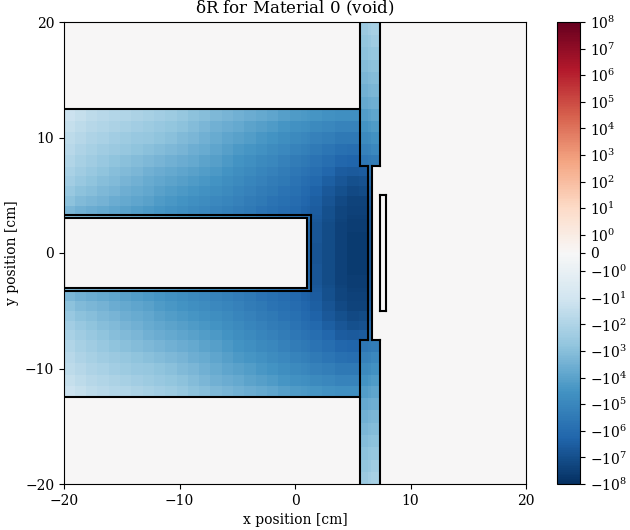
\includegraphics[width=\linewidth]{content/testprob/dR_00.png}
    \caption{$\delta R$ for void.}
    \label{fig:tp:dR_00}
  \end{minipage}
  \hfill
  \begin{minipage}{0.49\linewidth}
    \centering
    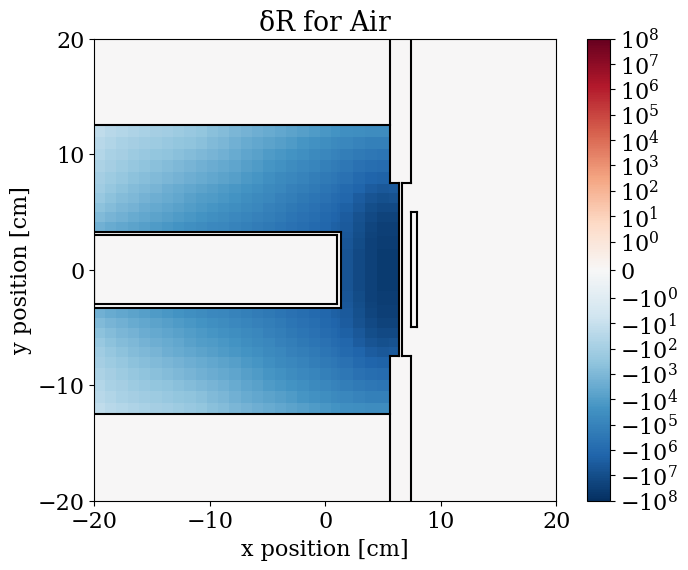
\includegraphics[width=\linewidth]{content/testprob/dR_01.png}
    \caption{$\delta R$ for air.}
    \label{fig:tp:dR_01}
  \end{minipage}
\end{figure}

Analysis for all subsequent plots will only focus on the moderating region (light blue region in \ref{fig:tp:material_map}) because the goal of the test problem is to construct the optimal moderator.

Plots of $\delta R$ for beryllium oxide (BeO) and graphite are shown in Figures \ref{fig:tp:dR_04} and \ref{fig:tp:dR_06}.
Both plots show that the detector response decreases if the material between the source and detector (the baseline is water) is replaced with the new material.
This implies that water is superior to both BeO and graphite in that region for the purposes of this problem.
There are regions in the water behind the source and far from the detector where $\delta R$ for BeO is slightly positive, however.
This indicates that the optimal moderator geometry would consist of two or more materials.

\begin{figure}
  \begin{minipage}{0.49\linewidth}
    \centering
    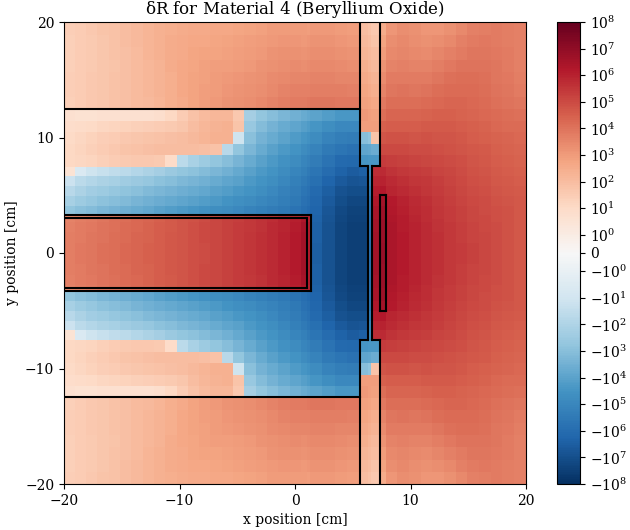
\includegraphics[width=\linewidth]{content/testprob/dR_04.png}
    \caption{$\delta R$ for beryllium oxide.}
    \label{fig:tp:dR_04}
  \end{minipage}
  \hfill
  \begin{minipage}{0.49\linewidth}
    \centering
    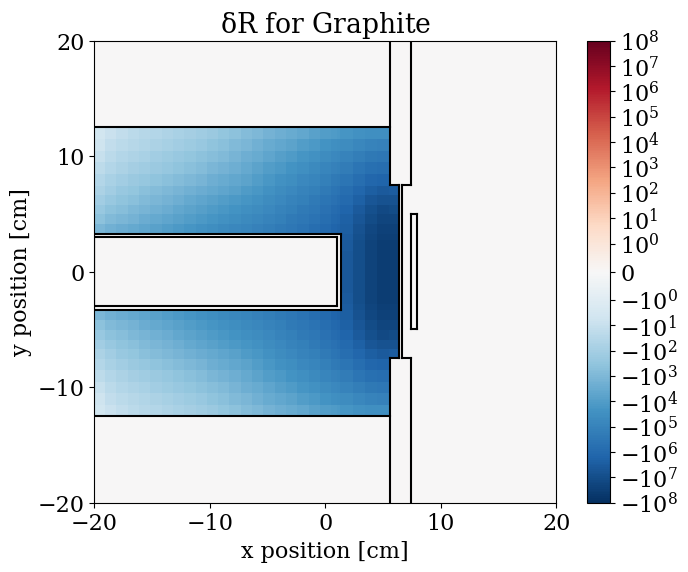
\includegraphics[width=\linewidth]{content/testprob/dR_06.png}
    \caption{$\delta R$ for graphite.}
    \label{fig:tp:dR_06}
  \end{minipage}
\end{figure}

Plots of $\delta R$ for water and heavy water are shown in Figures \ref{fig:tp:dR_12} and \ref{fig:tp:dR_11}.
Understandably, the plot for water does not provide any useful information: all it shows is that replacing water with itself does not change the detector response.
The plot for heavy water shows that it is worse than water at every location in the moderator.
This makes sense because more scattering events are required to thermalize neutrons with deuterium than are required with regular hydrogen.

\begin{figure}
  \begin{minipage}{0.49\linewidth}
    \centering
    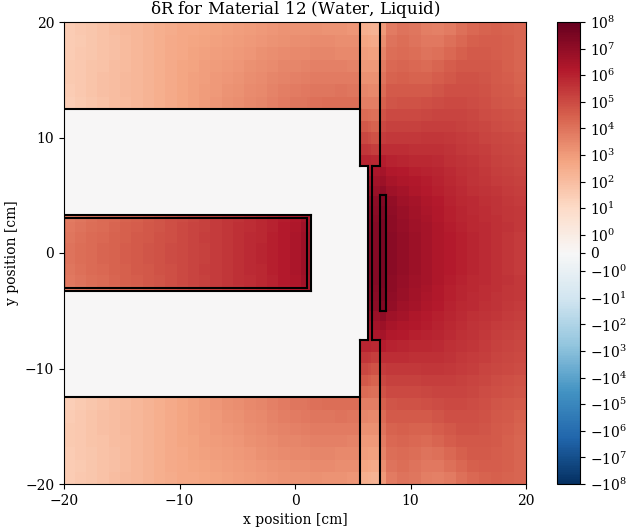
\includegraphics[width=\linewidth]{content/testprob/dR_12.png}
    \caption{$\delta R$ for water.}
    \label{fig:tp:dR_12}
  \end{minipage}
  \hfill
  \begin{minipage}{0.49\linewidth}
    \centering
    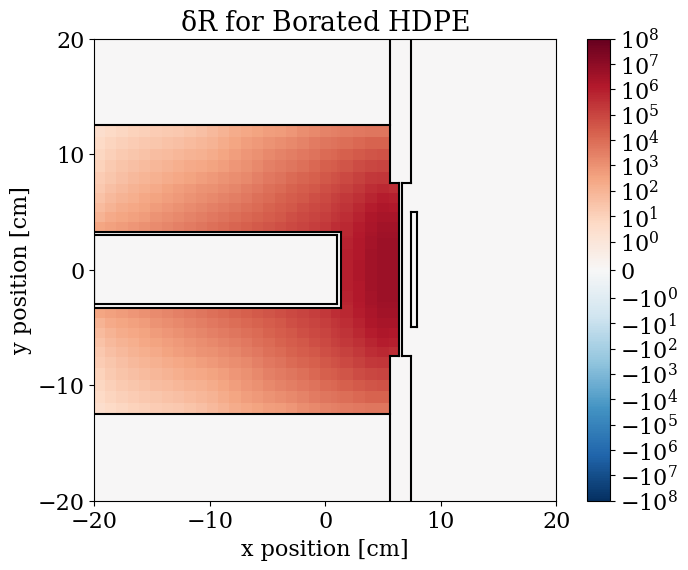
\includegraphics[width=\linewidth]{content/testprob/dR_11.png}
    \caption{$\delta R$ for heavy water.}
    \label{fig:tp:dR_11}
  \end{minipage}
\end{figure}

Plots of $\delta R$ for polyethylene (HDPE) and borated HDPE are shown in Figures \ref{fig:tp:dR_10} and \ref{fig:tp:dR_09}.
These plots show that both materials are superior to water at every location in the moderator.
The HDPE result makes sense because HDPE has a higher hydrogen density than water, meaning it can thermalize neutrons in shorter distances.
The borated HDPE result does not make much sense because boron has an extremely high absorption cross section for thermal neutrons, which intuitively should result in a decrease in the detector response.
More analysis is needed on this subject.

\begin{figure}
  \begin{minipage}{0.49\linewidth}
    \centering
    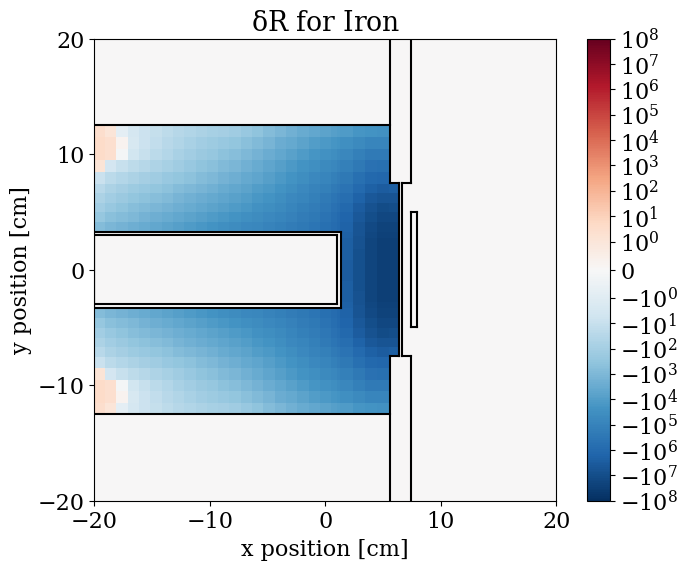
\includegraphics[width=\linewidth]{content/testprob/dR_10.png}
    \caption{$\delta R$ for polyethylene.}
    \label{fig:tp:dR_10}
  \end{minipage}
  \hfill
  \begin{minipage}{0.49\linewidth}
    \centering
    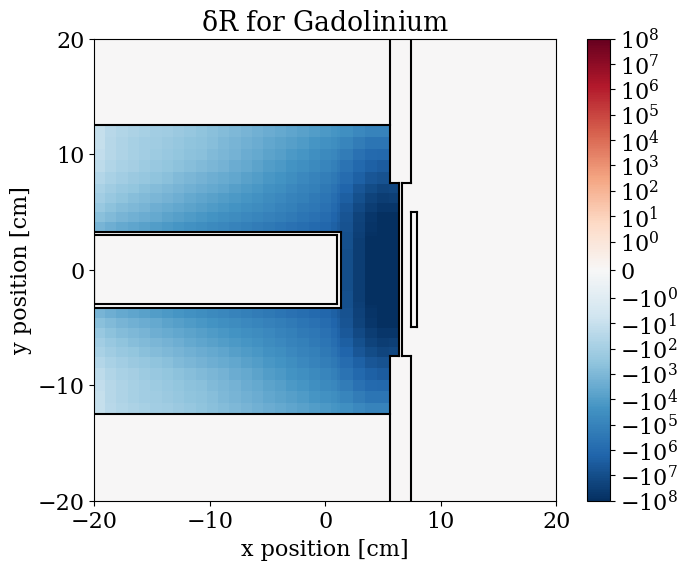
\includegraphics[width=\linewidth]{content/testprob/dR_09.png}
    \caption{$\delta R$ for borated polyethylene.}
    \label{fig:tp:dR_09}
  \end{minipage}
\end{figure}

Plots of $\delta R$ for aluminum, iron, boron, and ${}^{235}\text{U}$ are shown in Figures \ref{fig:tp:dR_02}, \ref{fig:tp:dR_08}, \ref{fig:tp:dR_05}, and \ref{fig:tp:dR_13}, respectively.
The plots show that all four materials perform considerably worse than water throughout the moderator, which makes sense because none of these materials are considered to be effective moderators.
The plot for ${}^{235}\text{U}$ does showcase one of the limitations of this approach: neutron multiplication due to fission is not taken into account.

\begin{figure}
  \begin{minipage}{0.49\linewidth}
    \centering
    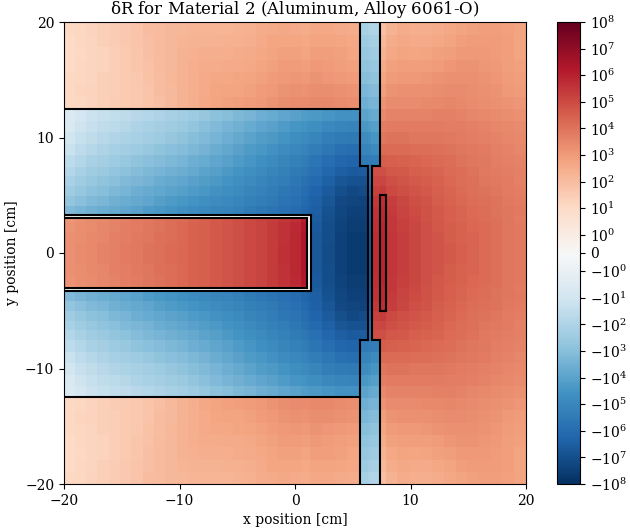
\includegraphics[width=\linewidth]{content/testprob/dR_02.png}
    \caption{$\delta R$ for aluminum.}
    \label{fig:tp:dR_02}
  \end{minipage}
  \hfill
  \begin{minipage}{0.49\linewidth}
    \centering
    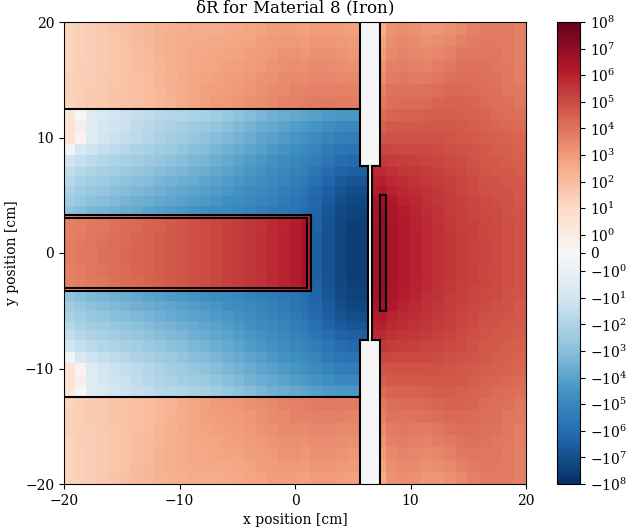
\includegraphics[width=\linewidth]{content/testprob/dR_08.png}
    \caption{$\delta R$ for iron.}
    \label{fig:tp:dR_08}
  \end{minipage}
\end{figure}
\begin{figure}
  \begin{minipage}{0.49\linewidth}
    \centering
    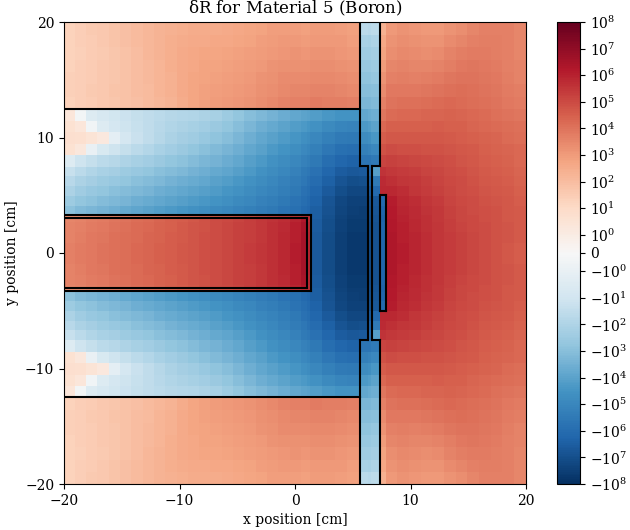
\includegraphics[width=\linewidth]{content/testprob/dR_05.png}
    \caption{$\delta R$ for boron.}
    \label{fig:tp:dR_05}
  \end{minipage}
  \hfill
  \begin{minipage}{0.49\linewidth}
    \centering
    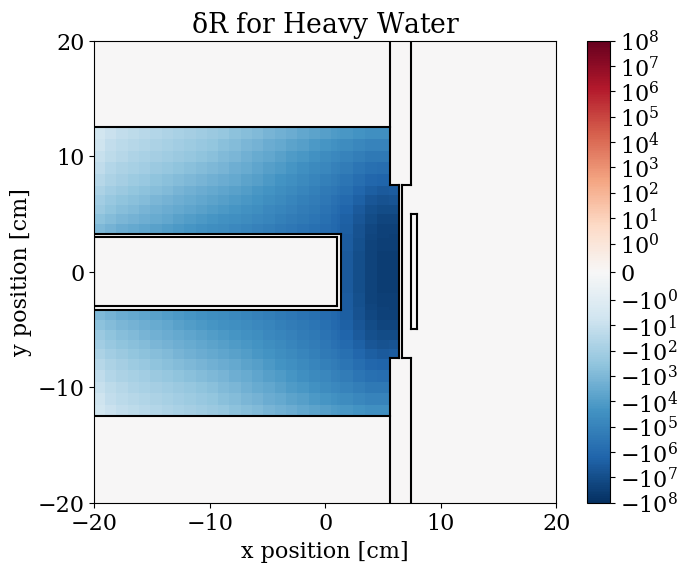
\includegraphics[width=\linewidth]{content/testprob/dR_13.png}
    \caption{$\delta R$ for ${}^{235}\text{U}$.}
    \label{fig:tp:dR_13}
  \end{minipage}
\end{figure}

%%%%%%%%%%%%%%%%%%%%%%%%%%%%%%%%%%%%%%%%%%%%%%%%%%%%%%%%%%%%%%%%%%%%%%%%%%%%%%%%
\section{MCNP Validation}
\label{sec:bg:tp:mcnp}
%%%%%%%%%%%%%%%%%%%%%%%%%%%%%%%%%%%%%%%%%%%%%%%%%%%%%%%%%%%%%%%%%%%%%%%%%%%%%%%%
